\documentclass[12pt]{article}
\usepackage[utf8]{inputenc}
\usepackage[spanish]{babel}
\usepackage{graphicx}
\usepackage{listings}
\usepackage{color}
\usepackage{hyperref}
\usepackage{caption}
\usepackage{float}
\usepackage{titlesec}
\usepackage{geometry}
\geometry{a4paper, margin=2.5cm}

% Configuración del paquete listings para mostrar código
\definecolor{codegray}{gray}{0.95}
\lstset{
    backgroundcolor=\color{codegray},
    basicstyle=\ttfamily\small,
    breaklines=true,
    frame=single,
    tabsize=4,
    showstringspaces=false,
    inputencoding=utf8,
    language=bash
}

\title{\textbf{Documentación del Proyecto}}
\author{Eduardo Yael Jiménez Sánchez}
\date{\today}

\begin{document}

\maketitle
\tableofcontents
\newpage

\section{Introducción}
El presente proyecto tiene como objetivo el desarrollo de una terminal de trabajo personalizada utilizando el lenguaje de scripting Bash en un entorno Linux. Esta terminal está pensada para brindar una experiencia de uso interactiva y adaptada a las necesidades del usuario, integrando comandos propios que permiten consultar información del sistema, gestionar tareas simples, ejecutar utilidades como un juego textual o un reproductor de música, y presentar mensajes personalizados con un enfoque educativo. \\

Desde el momento en que el usuario accede a la terminal, se desactiva el uso de combinaciones de teclado como Ctrl+C y Ctrl+Z, con el fin de mantener el flujo de ejecución controlado. El entorno muestra una interfaz personalizada con arte ASCII y un mensaje de bienvenida que invita al usuario a interactuar con los distintos comandos disponibles. Entre estos comandos se encuentran funciones para visualizar la fecha actual, información del sistema, créditos del proyecto, un juego tipo ahorcado, un reproductor de archivos MP3 con interfaz gráfica, y una sección de ayuda que explica el uso de cada uno de ellos.

\section{Desarrollo}

A continuación se explican los scripts principales del proyecto, incluyendo capturas de pantalla de su ejecución y el código correspondiente.

\subsection{main.sh}
Script principal que inicia el entorno de la terminal.

\begin{lstlisting}[caption={main.sh}]
#!/bin/bash

./login.sh

if [ $? -eq 0 ]; then
    ./terminal.sh
else
    echo "Error al iniciar sesion. Saliendo."
    exit 1
fi
\end{lstlisting}

\begin{figure}[H]
    \centering
    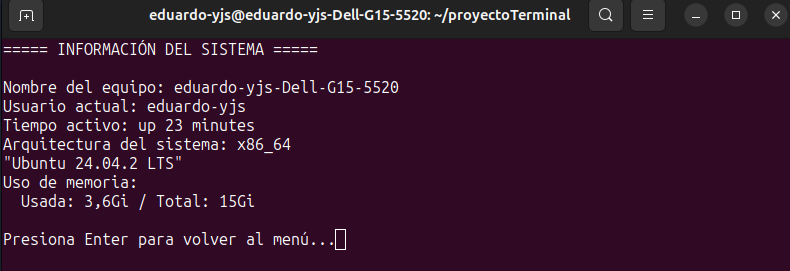
\includegraphics[width=0.8\textwidth]{capturas/infosis_ejecucion.png}
    \caption{Ejecución del script infosis.sh}
\end{figure}

\subsection{terminal.sh}
Shell personalizado que interpreta los comandos ingresados por el usuario.

\begin{lstlisting}[caption={shell.sh}]
#!/bin/bash
clear
echo "Bienvenido a la terminal personalizada"
while true; do
    echo -n "$USER@custom-terminal:~$ "
    read comando
    case $comando in
        login) bash login.sh ;;
        ayuda) bash ayuda.sh ;;
        infosis) bash infosis.sh ;;
        fecha) bash fecha.sh ;;
        buscar) bash buscar.sh ;;
        creditos) bash creditos.sh ;;
        juego) bash juego.sh ;;
        musica) bash reproductor.sh ;;
        salir) break ;;
        *) echo "Comando no reconocido" ;;
    esac
done
\end{lstlisting}

\begin{figure}[H]
    \centering
    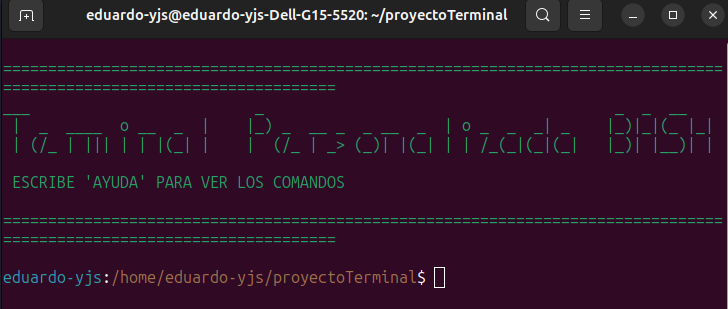
\includegraphics[width=0.8\textwidth]{capturas/terminal_ejecucion.png}
    \caption{Ejecución del shell personalizado}
\end{figure}

\subsection{login.sh}
Comando que permite acceder a la terminal con un usuario y contraseña existentes en el SO.

\begin{lstlisting}[caption={login.sh}]
#!/bin/bash
echo "Bienvenido a la terminal"

# Leer usuario y contraseña (con read -s, luego un echo para el salto)
read -p "Usuario: " usuario
read -s -p "Contraseña: " clave
echo

# Verificar si el usuario existe
if ! id "$usuario" &>/dev/null; then
    echo "Usuario no encontrado"
    exit 1
fi
# Comprobar la contraseña mediante el comando passwd
echo "$clave" | su - "$usuario" -c "exit" &>/dev/null
# Verificar si la contraseña fue correcta
if [ $? -eq 0 ]; then
    echo "Acceso concedido. Bienvenido $usuario"
    exit 0
else
    echo "Contraseña incorrecta"
    exit 1
fi
\end{lstlisting}

\begin{figure}[H]
    \centering
    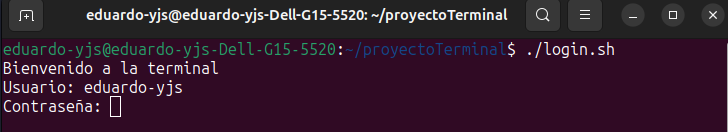
\includegraphics[width=0.8\textwidth]{capturas/login_ejecucion.png}
    \caption{Ejecución de login.sh}
\end{figure}


\newpage
\subsection{ayuda.sh}

Muestra una lista de los comandos personalizados dosponibles.

\begin{lstlisting}[caption={ayuda.sh}]
echo
echo "--------------------------------------------------------"
echo "      Lista de comandos"
echo "--------------------------------------------------------"
echo "ayuda         ->      muestra comandos"
echo "buscar        ->      buscar un archivo en un directorio (carpeta a buscar , archivo que va a buscar)"
echo "creditos      ->      muestra creditos de los creadores"
echo "fecha         ->      muestra la fecha y hora"
echo "infosis       ->      muestra informacion del sistema"
echo "ahorcado      ->      pasar un buen rato jugando ahorcado"
echo "reproductor   ->      reproductor de musica (Presiona Q para detener la musica)"
echo "Salir         ->      salir de la terminal"

\end{lstlisting}

\begin{figure}[H]
    \centering
    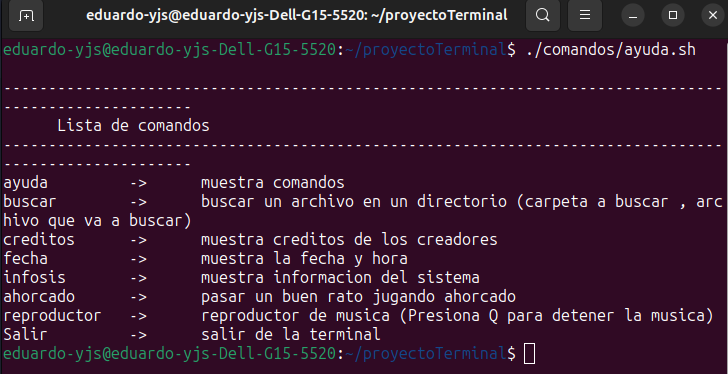
\includegraphics[width=0.8\textwidth]{capturas/ayuda_ejecucion.png}
    \caption{Ejecución de ayuda.sh}
\end{figure}


\newpage
\subsection{infosis.sh}
Muestra informacion del sistema (RAM, arquitectura del sistema y version del SO).

\begin{lstlisting}[caption={infosis.sh}]
#!/bin/bash
clear
echo "===== INFORMACIÓN DEL SISTEMA ====="
echo
# Nombre del equipo
echo "Nombre del equipo: $(hostname)"
# Nombre del usuario
echo "Usuario actual: $USER"
# Tiempo activo del sistema
echo "Tiempo activo: $(uptime -p)"
# Arquitectura del sistema
echo "Arquitectura del sistema: $(uname -m)"
# Sistema operativo y versión
grep "PRETTY_NAME" /etc/os-release | cut -d= -f2
# Uso de memoria
echo "Uso de memoria:"
free -h | awk 'NR==2{printf "  Usada: %s / Total: %s\n", $3, $2}'
echo
read -p "Presiona Enter para volver al menú..."

\end{lstlisting}

\begin{figure}[H]
    \centering
    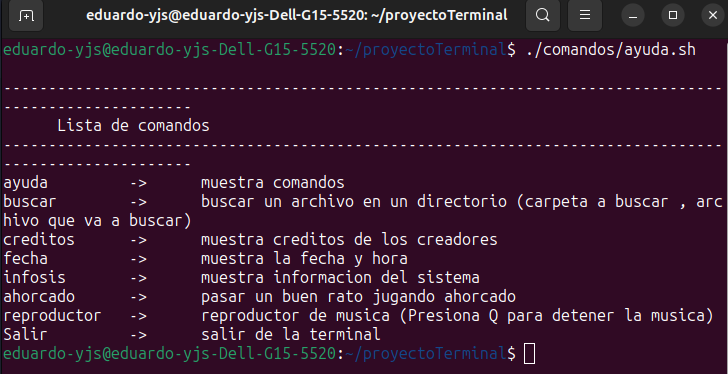
\includegraphics[width=0.8\textwidth]{capturas/ayuda_ejecucion.png}
    \caption{Ejecución de ayuda.sh}
\end{figure}


\newpage
\subsection{fecha.sh}
Muestra la fecha y hora actual.

\begin{lstlisting}[caption={fecha.sh}]
#!/bin/bash
#Comando para ajustar a la hora local: sudo timedatectl set-local-rtc 1
# Función para obtener fecha y hora desde RTC
obtener_fecha_hora() {
    local rtc_file="/proc/driver/rtc"
    local fecha_hora hora
    
    # Verificar si existe el archivo RTC
    if [[ ! -f "$rtc_file" ]]; then
        echo "Error: No se encontró el archivo RTC" >&2
        return 1
    fi

    # Extraer fecha y hora
    fecha_hora=$(awk '/rtc_date/ {print $3}' "$rtc_file" 2>/dev/null)
    hora=$(awk '/rtc_time/ {print $3}' "$rtc_file" 2>/dev/null)

    # Mostrar resultados
    printf "Fecha: %s\n" "$fecha_hora"
    printf "Hora: %s\n" "$hora"
}

# Llamar a la función principal
obtener_fecha_hora
\end{lstlisting}

\begin{figure}[H]
    \centering
    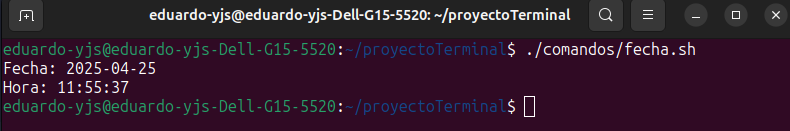
\includegraphics[width=0.8\textwidth]{capturas/fecha_ejecucion.png}
    \caption{Ejecución de fecha.sh}
\end{figure}


\newpage
\subsection{buscar.sh}
Busca un archivo en un directorio específico, recibe dos parámetros: La carpeta a buscar y el archivo que va a buscar.

\begin{lstlisting}[caption={buscar.sh}]
#!/bin/bash

# Pedir al usuario que ingrese el directorio y el archivo
read -p "Ingrese el directorio donde buscar (ruta): " directorio
read -p "Ingrese el nombre del archivo a buscar: " archivo

# Verificar si el directorio existe
if [ ! -d "$directorio" ]; then
    echo "ERROR: El directorio '$directorio' no existe."
    exit 1
fi

# Buscar el archivo en el directorio
busqueda=$(find "$directorio" -name "$archivo" 2>/dev/null)

# Comprobar si el archivo fue encontrado
if [ -z "$busqueda" ]; then
    echo "ERROR: El archivo '$archivo' no existe en '$directorio'."
    exit 1
else
    echo "Archivo '$archivo' encontrado en:"
    echo "$busqueda"
fi
\end{lstlisting}

\begin{figure}[H]
    \centering
    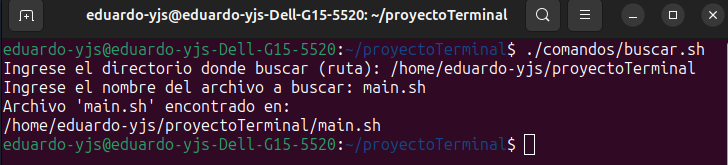
\includegraphics[width=0.8\textwidth]{capturas/buscar_ejecucion.png}
    \caption{Ejecución de buscar.sh}
\end{figure}


\newpage
\subsection{creditos.sh}
Muestra los créditos.

\begin{lstlisting}[caption={creditos.sh}]
#!/bin/bash
# Limpiar pantalla antes de mostrar (opcional)
clear
# Arte ASCII personalizado
echo -e "${GREEN}"
cat << "EOF"
                                            
  ,----..                                         ___                          
 /   /   \                        ,---,  ,--,   ,--.'|_                        
|   :     :  __  ,-.            ,---.'|,--.'|   |  | :,'   ,---.               
.   |  ;. /,' ,'/ /|            |   | :|  |,    :  : ' :  '   ,'\   .--.--.    
.   ; /-- '  | |' | ,---.      |   | |--'_  .;__,'  /  /   /   | /  /    '   
;   | ;    |  |   ,'/     \   ,--.__| |,' ,'| |  |   |  .   ; ,. :|  :  /./   
|   : |    '  :  / /    /  | /   ,'   |'  | | :__,'| :  '   | |: :|  :  ;_     
.   | '___ |  | ' .    ' / |.   '  /  ||  | :   '  : |__'   | .; : \  \    .  
'   ; : .'|;  : | '   ;   /|'   ; |:  |'  : |__ |  | '.'|   :    |  ----.   \ 
'   | '/  :|  , ; '   |  / ||   | '/  '|  | '.'|;  :    ;\   \  /  /  /--'  / 
|   :    /  ---'  |   :    ||   :    :|;  :    ;|  ,   /  ----'  '--'.     /  
 \   \ .'          \   \  /  \   \  /  |  ,   /  ----'             --'---'   
  ---             ----'    ----'    ----'                                 
   ___  ___  ______  _____________________    _________  _____   __     __   _____  ____  ___  __
  / _ \/ _ \/ __ \ \/ / __/ ___/_  __/ __ \  / __/  _/ |/ / _ | / /    / /  /  _/ |/ / / / / |/_/
 / ___/ , _/ /_/ /\  / _// /__  / / / /_/ / / _/_/ //    / __ |/ /__  / /___/ //    / /_/ />  <  
/_/  /_/|_|\____/ /_/___/\___/ /_/  \____/ /_/ /___/_/|_/_/ |_/____/ /____/___/_/|_/\____/_/|_|  
   ___                           ____        __                     _                                               
  / _ \___ ______ ____________  / / /__ ____/ /__    ___  ___  ____(_)                                              
 / // / -_|_-< _ / __/ __/ _ \/ / / _ / _  / _ \  / _ \/ _ \/ __/                                                 
/____/\__/___|_,_/_/ /_/  \___/_/_/\_,_/\_,_/\___/ / .__/\___/_/ (_)                                                
   ____   __                 __                     __    _ _                          ____              __         
  / __/__/ /_ _____ ________/ /__    __ _____ ____ / /   (_|_)_ _  ___ ___  ___ ___   / __/__ ____  ____/ /  ___ ___
 / _// _  / // / _ / __/ _  / _ \  / // / _ / -_) /   / / /  ' \/ -_) _ \/ -_)_ /  _\ \/ _ / _ \/ __/ _ \/ -_)_ /
/___/\_,_/\_,_/\_,_/_/  \_,_/\___/  \_, /\_,_/\__/_/ __/ /_/_/_/_/\__/_//_/\__//__/ /___/\_,_/_//_/\__/_//_/\__//__/
                                   /___/            |___/                     
   _______   _  __
  /  _/ _ | / |/ /
 _/ // __ |/    / 
/___/_/ |_/_/|_/  
  _____             _                   ___  ___  ____  ______________________     
 / ___/______ _____(_)__ ____   ___ _  / _ \/ _ \/ __ \/_  __/ __/ ___/ __/ _ |    
/ (_ / __/ _ / __/ / _ (_-<  / _ / / ___/ , _/ /_/ / / / / _// /___\ \/ __ |    
\___/_/  \_,_/\__/_/\_,_/___/  \_,_/ /_/  /_/|_|\____/ /_/ /___/\___/___/_/ |_|    
                 __           _         __               __                        
  __ __  ___ _  / /__  ___   (_)__  ___/ /_______ ______/ /____  _______ ___       
 / // / / _ / / / _ \(_-<  / / _ \(_-< __/ __/ // / __/ __/ _ \/ __/ -_|_-<       
 \_, /  \_,_/ /_/\___/___/ /_/_//_/___|__/_/  \_,_/\__/\__/\___/_/  \__/___/       
/___/                                                                              
EOF
echo
read -p "Presiona Enter para volver al menú..."
\end{lstlisting}

\begin{figure}[H]
    \centering
    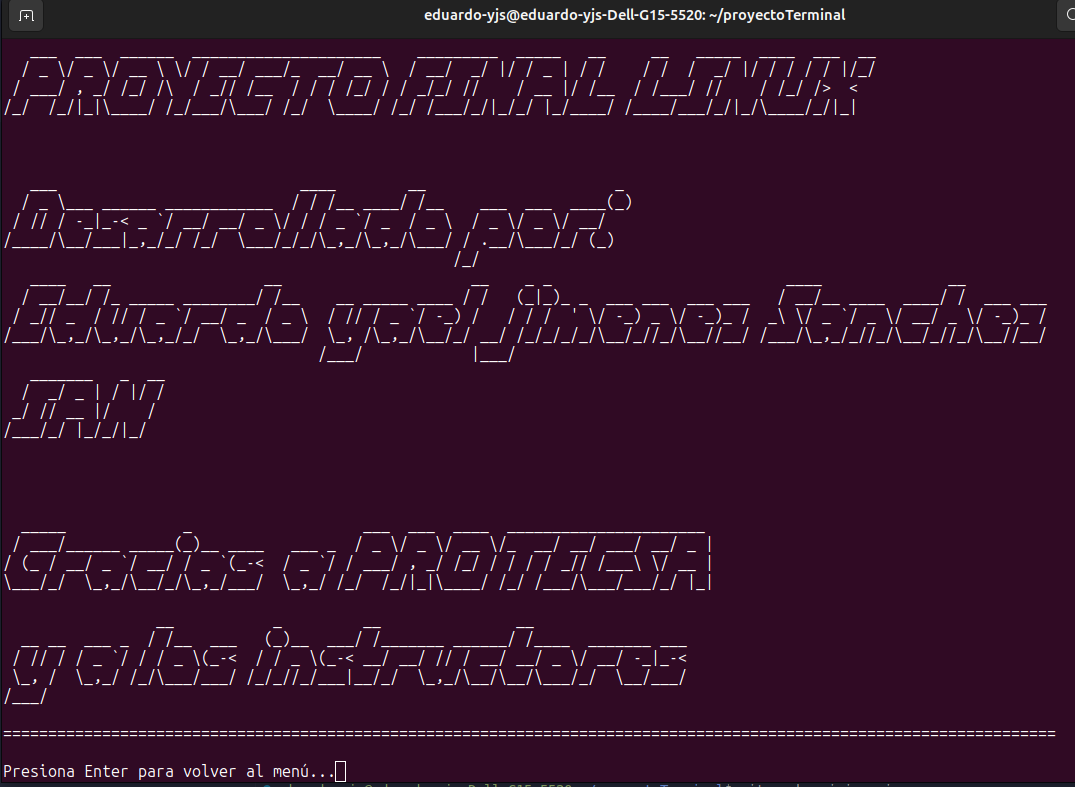
\includegraphics[width=0.8\textwidth]{capturas/creditos_ejecucion.png}
    \caption{Ejecución de creditos.sh}
\end{figure}

\newpage
\subsection{juego.sh}
Despliega un juego en la terminal (Ahorcado).

\begin{lstlisting}[caption={Ahorcado.sh}]
#!/bin/bash

# Juego del Ahorcado simplificado

# Palabra secreta
palabra="programacion"
intentos=6
letras_adivinadas=()
letras_incorrectas=()

# Dibujar el ahorcado según intentos restantes
dibujar_ahorcado() {
    case $intentos in
        6) echo "  _____"; echo " |    "; echo " |    "; echo " |    "; echo "_|____";;
        5) echo "  _____"; echo " |    O"; echo " |    "; echo " |    "; echo "_|____";;
        4) echo "  _____"; echo " |    O"; echo " |    |"; echo " |    "; echo "_|____";;
        3) echo "  _____"; echo " |    O"; echo " |   /|"; echo " |    "; echo "_|____";;
        2) echo "  _____"; echo " |    O"; echo " |   /|\\"; echo " |    "; echo "_|____";;
        1) echo "  _____"; echo " |    O"; echo " |   /|\\"; echo " |   / "; echo "_|____";;
        0) echo "  _____"; echo " |    O"; echo " |   /|\\"; echo " |   / \\"; echo "_|____";;
    esac
}

# Mostrar la palabra con letras adivinadas
mostrar_palabra() {
    for ((i=0; i<${#palabra}; i++)); do
        letra=${palabra:i:1}
        [[ " ${letras_adivinadas[@]} " =~ " $letra " ]] && echo -n "$letra" || echo -n "_"
    done
    echo
}

# Bucle principal
while (( intentos > 0 )); do
    clear
    echo "=== AHORCADO ==="
    dibujar_ahorcado
    echo
    echo "Palabra: $(mostrar_palabra)"
    echo "Intentos restantes: $intentos"
    echo "Letras incorrectas: ${letras_incorrectas[*]}"
    # Verificar si ganó
    if ! mostrar_palabra | grep -q "_"; then
        echo "¡Ganaste! La palabra era: $palabra"
        exit 0
    fi
    # Pedir letra
    read -p "Introduce una letra: " -n 1 letra
    echo
    # Validar letra
    if [[ " ${letras_adivinadas[@]} ${letras_incorrectas[@]} " =~ " $letra " ]]; then
        echo "Ya usaste esa letra"
        sleep 1
        continue
    fi
    # Verificar letra
    if [[ "$palabra" == *"$letra"* ]]; then
        letras_adivinadas+=("$letra")
        echo "¡Correcto!"
    else
        letras_incorrectas+=("$letra")
        ((intentos--))
        echo "Incorrecto"
    fi
    sleep 1
done
# Si llega aquí, perdió
clear
dibujar_ahorcado
echo "¡Perdiste! La palabra era: $palabra"

\end{lstlisting}

\begin{figure}[H]
    \centering
    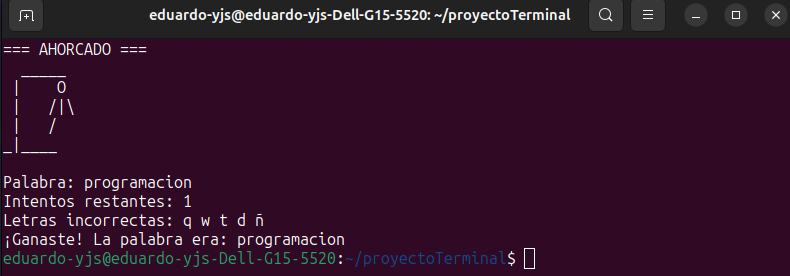
\includegraphics[width=0.8\textwidth]{capturas/juego_ejecucion.png}
    \caption{Ejecución de ahorcado.sh}
\end{figure}

\newpage
\subsection{reproductor.sh}
Reproductor MP3 con interfaz gráfica.

\begin{lstlisting}[caption={mp3Player.sh}]
#!/bin/bash

# Reproductor de Música Avanzado
# Versión mejorada con interfaz gráfica y más funcionalidades

# Configuración inicial
carpeta_musica="/home/eduardo-yjs/proyectoTerminal/musica"
temp_file="/tmp/music_player_temp.txt"
icono_reproductor="audio-x-generic"
player_command="mpg123"  # Puedes cambiarlo por tu reproductor preferido (mpg123, mplayer, etc.)

# Verificar dependencias
if ! command -v zenity &> /dev/null || ! command -v $player_command &> /dev/null; then
    echo "Error: Necesitas instalar zenity y $player_command para usar este reproductor."
    echo "En Ubuntu/Debian puedes instalarlos con:"
    echo "sudo apt install zenity mpg123"
    exit 1
fi

# Función para obtener la lista de canciones
obtener_canciones() {
    find "$carpeta_musica" -type f \( -iname "*.mp3" -o -iname "*.ogg" -o -iname "*.wav" \) | sort
}

# Función para mostrar el menú principal
mostrar_menu_principal() {
    zenity --list \
        --title="Reproductor de Música" \
        --text="Selecciona una opción:" \
        --column="Opción" \
        --width=500 \
        --height=300 \
        --window-icon="$icono_reproductor" \
        "Reproducir canción" \
        "Lista de reproducción" \
        "Reproducir aleatorio" \
        "Buscar canción" \
        "Información del reproductor" \
        "Salir"
}

# Función para mostrar la lista de canciones con selección
mostrar_lista_canciones() {
    canciones=$(obtener_canciones)
    if [ -z "$canciones" ]; then
        zenity --error \
            --title="Error" \
            --text="No se encontraron canciones en $carpeta_musica" \
            --width=300
        return 1
    fi
    
    # Mostrar lista con nombres de archivo sin la ruta
    (IFS=$'\n'; zenity --list \
        --title="Selecciona una canción" \
        --text="Canciones disponibles:" \
        --column="Canciones" \
        --width=600 \
        --height=400 \
        --window-icon="$icono_reproductor" \
        $(while read -r cancion; do basename "$cancion"; done <<< "$canciones"))
}

# Función para reproducir una canción
reproducir_cancion() {
    local cancion="$1"
    if [ ! -f "$cancion" ]; then
        zenity --error \
            --title="Error" \
            --text="No se pudo encontrar la canción: $cancion" \
            --width=400
        return 1
    fi
    
    # Mostrar información de la canción que se está reproduciendo
    (
        zenity --info \
            --title="Reproduciendo" \
            --text="Reproduciendo:\n$(basename "$cancion")" \
            --width=400 \
            --height=150 \
            --window-icon="$icono_reproductor" &
    ) 2>/dev/null
    
    # Reproducir la canción
    $player_command "$cancion" 2>/dev/null
    
    # Cerrar la ventana de información después de la reproducción
    pkill -f "zenity --info.*Reproduciendo"
}

# Función para crear una lista de reproducción
crear_lista_reproduccion() {
    canciones=$(obtener_canciones)
    if [ -z "$canciones" ]; then
        zenity --error \
            --title="Error" \
            --text="No se encontraron canciones para crear la lista" \
            --width=300
        return 1
    fi
    
    # Guardar lista temporalmente
    echo "$canciones" > "$temp_file"
    
    zenity --info \
        --title="Lista de reproducción creada" \
        --text="Se ha creado una lista con ${#canciones[@]} canciones" \
        --width=300
}

# Función para reproducir la lista de reproducción
reproducir_lista() {
    if [ ! -f "$temp_file" ]; then
        zenity --error \
            --title="Error" \
            --text="No hay lista de reproducción creada" \
            --width=300
        return 1
    fi
    
    while read -r cancion; do
        reproducir_cancion "$cancion"
    done < "$temp_file"
}

# Función para reproducir en modo aleatorio
reproducir_aleatorio() {
    canciones=($(obtener_canciones | shuf))
    if [ ${#canciones[@]} -eq 0 ]; then
        zenity --error \
            --title="Error" \
            --text="No se encontraron canciones para reproducir" \
            --width=300
        return 1
    fi
    
    for cancion in "${canciones[@]}"; do
        reproducir_cancion "$cancion"
    done
}

# Función para buscar canciones
buscar_cancion() {
    termino=$(zenity --entry \
        --title="Buscar canción" \
        --text="Introduce el nombre de la canción:" \
        --width=400)
    
    if [ -z "$termino" ]; then
        return 1
    fi
    
    resultados=$(obtener_canciones | grep -i "$termino")
    if [ -z "$resultados" ]; then
        zenity --info \
            --title="Resultados de búsqueda" \
            --text="No se encontraron canciones con '$termino'" \
            --width=300
        return 1
    fi
    
    seleccion=$(IFS=$'\n'; zenity --list \
        --title="Resultados de búsqueda" \
        --text="Canciones encontradas:" \
        --column="Canciones" \
        --width=600 \
        --height=400 \
        $(while read -r cancion; do basename "$cancion"; done <<< "$resultados"))
    
    if [ -n "$seleccion" ]; then
        cancion=$(echo "$resultados" | grep -i -m1 "$seleccion")
        reproducir_cancion "$cancion"
    fi
}

# Función para mostrar información del reproductor
mostrar_info() {
    total_canciones=$(obtener_canciones | wc -l)
    zenity --info \
        --title="Información del Reproductor" \
        --text="Reproductor de Música\n\nVersión: 2.0\nCarpeta de música: $carpeta_musica\nCanciones disponibles: $total_canciones" \
        --width=400 \
        --height=200 \
        --window-icon="$icono_reproductor"
}

# Bucle principal del reproductor
while true; do
    opcion=$(mostrar_menu_principal)
    
    case "$opcion" in
        "Reproducir canción")
            cancion_seleccionada=$(mostrar_lista_canciones)
            if [ -n "$cancion_seleccionada" ]; then
                # Obtener la ruta completa de la canción seleccionada
                cancion=$(obtener_canciones | grep -i -m1 "$cancion_seleccionada")
                reproducir_cancion "$cancion"
            fi
            ;;
        "Lista de reproducción")
            crear_lista_reproduccion && reproducir_lista
            ;;
        "Reproducir aleatorio")
            reproducir_aleatorio
            ;;
        "Buscar canción")
            buscar_cancion
            ;;
        "Información del reproductor")
            mostrar_info
            ;;
        "Salir"|"")
            exit 0
            ;;
        *)
            zenity --error \
                --title="Error" \
                --text="Opción no válida" \
                --width=300
            ;;
    esac
done
\end{lstlisting}

\begin{figure}[H]
    \centering
    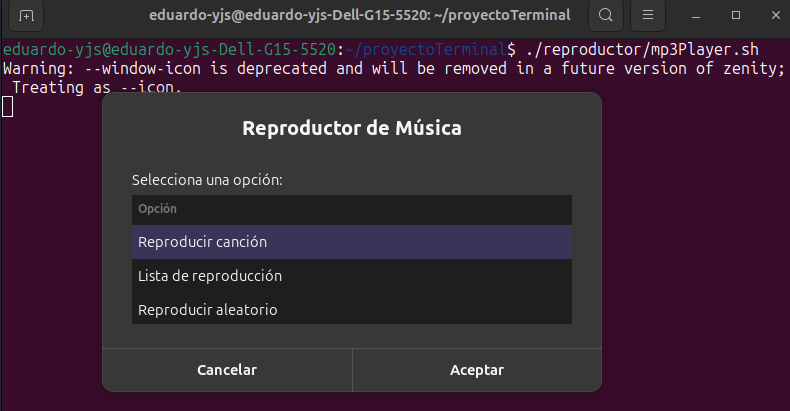
\includegraphics[width=0.8\textwidth]{capturas/reproductor_ejecucion.png}
    \caption{Ejecución de mp3Player.sh}
\end{figure}

\newpage
\section{Conclusiones}

\textbf{Eduardo Jiménez:} Desarrollar este proyecto fue una experiencia enriquecedora que me permitió poner en práctica y consolidar mis conocimientos en Bash y en el entorno del sistema operativo Linux. A lo largo del proceso, aprendí a estructurar scripts de manera lógica y eficiente, a manejar correctamente la entrada del usuario, y a aplicar colores y mensajes personalizados para mejorar la experiencia en la línea de comandos.

Uno de los aspectos que más disfruté fue integrar utilidades como un juego interactivo, ya que me permitió combinar habilidades técnicas con elementos creativos. También comprendí la importancia de mantener el código modular y bien organizado, lo cual facilitó tanto las pruebas como la escalabilidad del sistema.

En resumen, este proyecto no solo fortaleció mis habilidades en scripting, sino que también despertó en mí un mayor interés por seguir explorando el desarrollo de herramientas personalizadas en Bash, con miras a crear entornos más completos, útiles y atractivos para el usuario final.\\

\textbf{Ian:}

\end{document}